%license:BSD-3-Clause
%copyright-holders:Michele Maione
%============================================================
%
%	Piattaforma di cloud gaming per giochi arcade
%
%============================================================
\chapter{Implementazione}
%In questa sezione si spiega come è stato affrontato il problema concettualmente, la soluzione logica che ne è seguita senza la documentazione.
%Si mostra il progetto dell'architettura del sistema con i vari moduli.
In questo capitolo verranno descritte le cinque fasi aggiuntive del cloud gaming e la loro implementazione in C++ come nuovi moduli del MAME: la cattura audio-video, la codifica, la trasmissione, la decodifica e la cattura dell'input utente. Il processo completo è mostrato in Fig. \ref{fig:decodificaFilmato}.

\begin{figure}[H]
	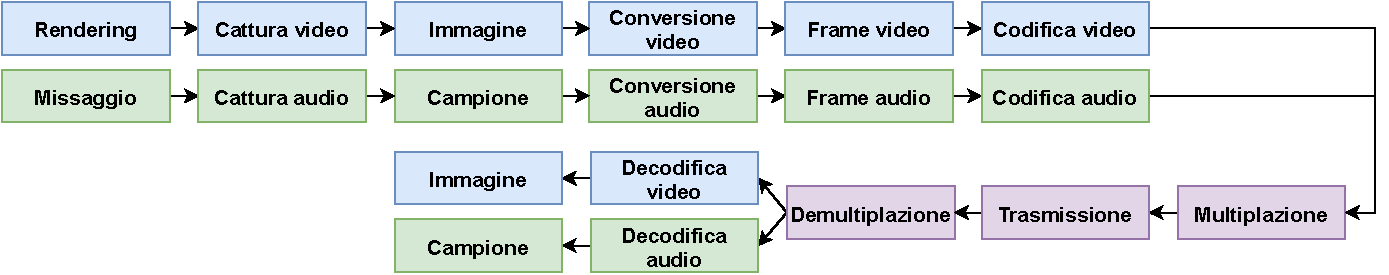
\includegraphics[width=\linewidth]{immagini/decodificaFilmato}
	\caption{Processo completo delle fasi del cloud gaming: dalla cattura audiovisiva alla visualizzazione}
	\label{fig:decodificaFilmato}
\end{figure}




\section{Cattura audiovisiva}
Nel paradigma del cloud gaming per cattura si intende la fase in cui l'output audiovisivo del videogioco non viene visualizzato (l'immagine) ed emesso (il suono) ma viene inviato ad un codificatore. Nei prossimi due paragrafi vedremo i metodi di cattura per la parte video e per quella audio.


\subsection{Cattura video} \label{subsec:cap3_Video}
Per la cattura video esistono tre metodi di cattura: l'hook di funzioni della libreria multimediale, l'utilizzo delle API per il framebuffer virtuale e l'uso di schede video con funzionalità di codifica incorporata.

L'hook di funzione è una tecnica di programmazione con la quale si sostituisce il comportamento di una funzione di un programma o di una libreria già compilata. Questa operazione su una libreria multimediale consiste nel modificare il normale funzionamento della procedura che invia il framebuffer della scheda video all'uscita. Ad esempio per le librerie multimediali più usate le funzioni da catturare sono: \verb|SDL_RenderPresent| per SDL, \verb|Present| per DirectX e \verb|SwapBuffer| per OpenGL \parencite{GamingAnywhere}. Questo metodo è stato usato ad esempio da OnLive, Gaikai e Vortex. Un esempio di codice per l'hook di funzioni per SDL è mostrato nel Lis. \ref{lst:hookCode}.

\begin{lstlisting}[caption=Codice di esempio per hook della libreria SDL, label={lst:hookCode}]
HOOK_TRACE_INFO hHook = { NULL };
HMODULE lib_handle = LoadLibrary("SDL2.dll");

FARPROC old_SDL_RenderPresent =	GetProcAddress(
	lib_handle, "SDL_RenderPresent");

NTSTATUS result = LhInstallHook(
	old_SDL_RenderPresent, my_SDL_RenderPresent,
	NULL, &hHook);
\end{lstlisting}

Il framebuffer virtuale è una funzionalità offerta dalle API di sistema per accedere all'attuale framebuffer presente nella scheda video. Il loro utilizzo principale è per il remote desktop, ma alcune piattaforme come "GamingAnywhere" \parencite{GamingAnywhere} e "Parsec"\footnote{Parsec è un servizio di desktop remoto basato su Windows offerto dalla omonima società.} \parencite{TheTechnologyBehindALowLatencyCloudGamingService} utilizzano questa funzionalità per la cattura video, il primo per la piattaforma di cloud gaming, il secondo per offrire un computer virtuale. Alcuni esempi nei moderni sistemi operativi sono: "X virtual framebuffer" del gestore grafico X11 su Linux \parencite{XVFB}, "Desktop Duplication API" su Windows \parencite{DesktopDuplicationAPI} e \verb|CGDisplayStream| della libreria "Quartz Display Services" su macOS.

Le schede video con codifica incorporata non hanno una fase di cattura poiché il chip di codifica legge i dati direttamente dal framebuffer; l'argomento è trattato più avanti nel paragrafo \ref{sec:cap3_Codifica}.

Poiché sono disponibili i sorgenti del progetto MAME in questo progetto ho scelto di modificare il comportamento normale del programma. Come mostrato in Fig. \ref{fig:class_renderingSDLFull_Streaming}, sono state aggiunte alla classe \verb|renderer_sdl2| le due funzioni (\verb|init_streaming_render| e \verb|free_streaming_render|) per allocare e deallocare le strutture dati per la cattura. Come mostrato nel Lis. \ref{lst:init_streaming_render_init} le funzioni della libreria SDL che sono state aggiunte al codice sono:

\begin{itemize}
	\item CreateRGBSurfaceWithFormat: crea una superficie RGB specificando il formato pixel da utilizzare;	
	\item CreateSoftwareRenderer: crea un contesto di rendering 2D per una superficie;
	\item RWFromMem: prepara un buffer di memoria di lettura-scrittura da utilizzare con la struttura dati RWops (read-write opaque pointer structure).	
\end{itemize}

\begin{lstlisting}[caption=Codice aggiunto per la cattura video: inizializzazione. File: \detokenize{osd/modules/render/draw13.cpp}, label={lst:init_streaming_render_init}]
sdl_buffer_bytes_length = w * h * 4; // RGBA = 4 bytes
sdl_buffer_bytes = new char[sdl_buffer_bytes_length];

sdl_surface = SDL_CreateRGBSurfaceWithFormat(
	0, w, h, 32, SDL_PIXELFORMAT_RGBA32);

sdl_renderer = SDL_CreateSoftwareRenderer(sdl_surface);
sdl_buffer = SDL_RWFromMem(
	sdl_buffer_bytes, sdl_buffer_bytes_length);
\end{lstlisting}

Nel Lis. \ref{lst:init_streaming_render_draw} è mostrato il codice che è stato inserito per inviare alla classe statica che gestisce lo streaming (\verb|streaming_server|) il frame da inviare al giocatore (che verrà codificato prima dell'invio). Poiché l'attuale contesto di rendering (\verb|sdl_renderer|) è creato su una superfice RGB (\verb|sdl_surface|) quando il contesto di rendering viene aggiornato con il framebuffer corrente (tramite \verb|SDL_RenderPresent|) è la superfice a ricevere il frame attuale.

\begin{lstlisting}[caption=Codice aggiunto per la cattura video: disegno. File: \detokenize{osd/modules/render/draw13.cpp}, label={lst:init_streaming_render_draw}]
SDL_RenderPresent(sdl_renderer);

streaming_server::instance()
	.send_video_frame(sdl_surface->pixels);

SDL_RWseek(sdl_buffer, 0, RW_SEEK_SET); // pos. inizio del buffer
\end{lstlisting}

\begin{figure}[H]
	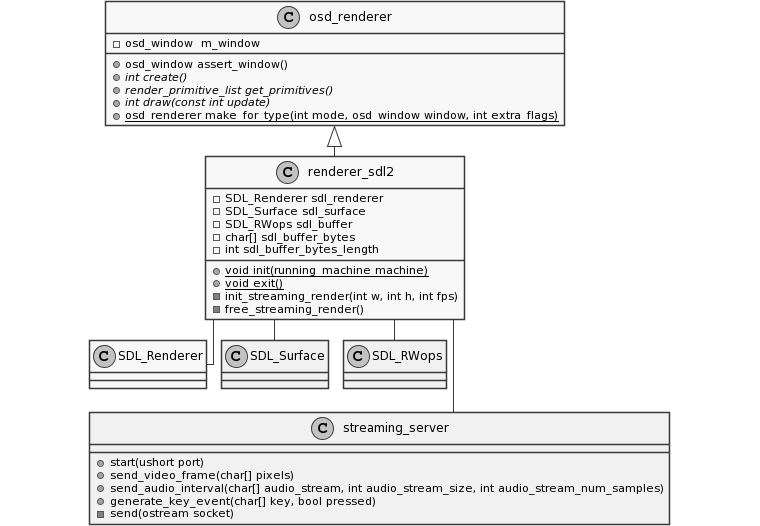
\includegraphics[width=\linewidth]{immagini/class_renderingSDLFull_Streaming}
	\caption{Diagramma delle classi relative alla cattura video}
	\label{fig:class_renderingSDLFull_Streaming}
\end{figure}



\subsection{Cattura audio} \label{subsec:cap3_Audio}
Come per la cattura video si può ricorrere all'hook di funzioni della libreria multimediale o alle API del sistema operativo per la gestione audio \parencite{GamingAnywhere}; ad esempio: "Windows Audio Session API" per Windows \parencite{WASAPI}, "Advanced Linux Sound Architecture" per Linux \parencite{ALSA} e "Core Audio" per macOS \parencite{Core_Audio_api}.

Come nel caso della cattura video ho scelto di modificare il sorgente del programma. Come mostrato in Fig. \ref{fig:class_mixingSDL_streaming} la classe \verb|sound_sdl| implementa la funzione di callback necessaria per utilizzare il missaggio audio di SDL, di cui abbiamo parlato nel paragrafo \ref{subsec:cap2_MissaggioAudio}. All'interno di questa funzione, tramite la funzione \verb|send_audio_interval|, è stato inviato alla classe che si occupa di gestire il server di streaming (\verb|streaming_server|) il buffer sonoro (\verb|stream|) e la sua dimensione (\verb|len|). La modifica apportata è mostrata nel Lis. \ref{lst:sdl_sound_callback}.

\begin{lstlisting}[caption=Codice aggiunto per la cattura audio. File: \detokenize{osd/modules/sound/sdl_sound.cpp}, label={lst:sdl_sound_callback}]
// 512 campioni audio (per canale)
streaming_server::instance()
	.send_audio_interval(stream, len, 512);

memset(stream, 0, len); // svuota buffer sonoro
\end{lstlisting}


\begin{figure}[H]
	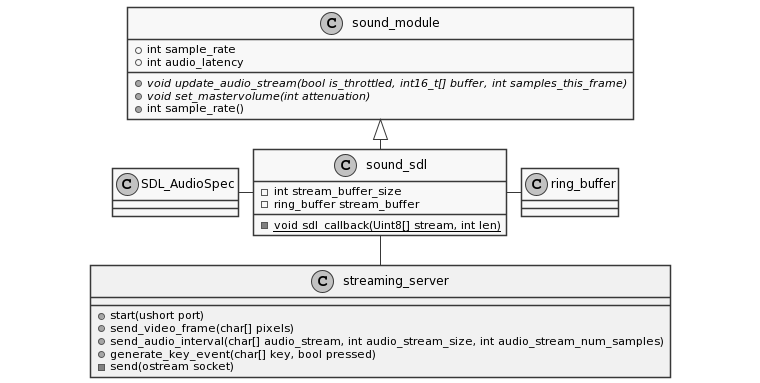
\includegraphics[width=\linewidth]{immagini/class_mixingSDL_streaming}
	\caption{Diagramma delle classi relative alla cattura audio}
	\label{fig:class_mixingSDL_streaming}
\end{figure}



\section{Codifica} \label{sec:cap3_Codifica}
Nel paradigma dello streaming la codifica è un processo essenziale sia perché stabilisce il formato audiovisivo che verrà trasmesso e poi decodificato sia perché riduce l'elevata quantità di dati che compongono il flusso audiovisivo. La codifica avviene tramite un codificatore (hardware o software) che descrive e comprime i dati (solitamente con perdita dell'informazione). Di seguito parleremo dei codificatori video e audio e di come è stata utilizzata la libreria FFmpeg per la codifica.

\subsection{Codificatori video}
I codificatori video si divino in due gruppi:

\begin{itemize}
	\item intraframe: codificano ogni fotogramma indipendentemente dagli altri;
	\item interframe: descrivono i cambiamenti tra fotogrammi contigui; sono più efficienti su scene statiche poiché i cambiamenti da descrivere sono minori.
\end{itemize}

%YUV 4:2:0 planare da 12bpp (1 Cr & Cb campioni per 2x2 Y campioni)
Gli attuali monitor (CRT, LCD, PDP e OLED) utilizzano RGB come modello di colori (e di conseguenza gli attuali sistemi operativi), ma gli algoritmi di codifica video utilizzano il modello YCbCr\footnote{Il termine YUV è usato molto spesso come sinonimo di YCbCr. Si tratta tuttavia di formati differenti, uno analogico e l'altro digitale.}. Sfruttando l'innata sensibilità alla luminosità del sistema visivo umano questo modello suddivide i dati del colore in componenti separati di luminanza e crominanza, come mostrato in Fig. \ref{fig:RGB_YCbCr}, possiamo comprimere selettivamente solo i componenti di crominanza per ottenere risparmi di spazio con una perdita minima di qualità.

Utilizzando le costanti dello standard NTSC e PAL: $K_R$, $K_G$ e $K_B$ che valgono rispettivamente $0.299$, $0.587$ e $0.114$ \parencite{VideoAndMultimediaTransmissionsOverCellularNetworks}, la conversione da YCbCr a RGB avviene utilizzando l'Eq. \ref{eq:YUV_from_RGB}:

\begin{equation} \label{eq:YUV_from_RGB}
	\begin{aligned}
		& Y = K_R R + K_G G + K_B B, \\	
		& C_B = \frac{0.5}{1 - K_B} (B - Y), \\
		& C_R = \frac{0.5}{1 - K_R} (R - Y).	
	\end{aligned}
\end{equation}

\begin{figure}[H]
	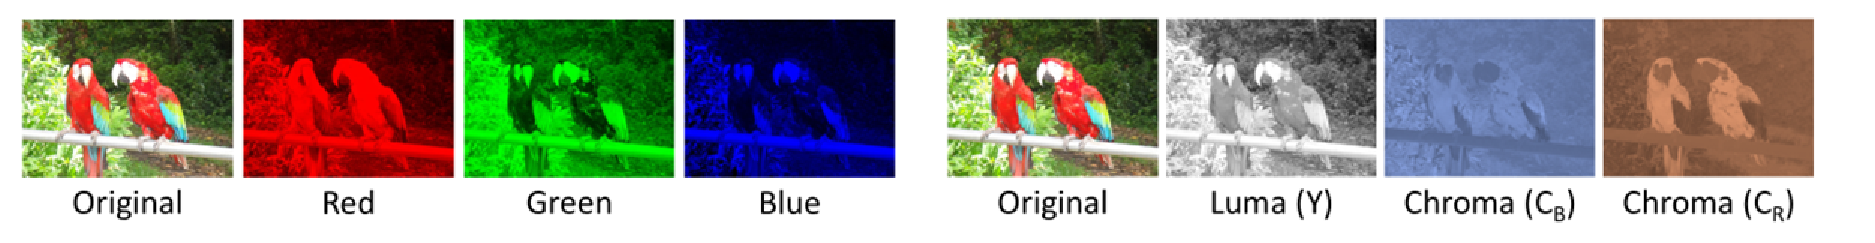
\includegraphics[width=\linewidth]{immagini/RGB_YCbCr}
	\caption{Componenti di RGB e YCbCr}
	\label{fig:RGB_YCbCr}
\end{figure}

Come mostrato in Fig. \ref{fig:RGB_YCbCr_matrix}, nel modello RGB i dati per un singolo componente di colore sono intercalati tra i pixel e ciascun pixel è archiviato in memoria in modo contiguo, mentre nel modello YCbCr le componenti Cb e Cr sono intercalate e memorizzate insieme, mentre la componente Y rimane nel proprio piano, per un totale di due piani.

\begin{figure}[H]
	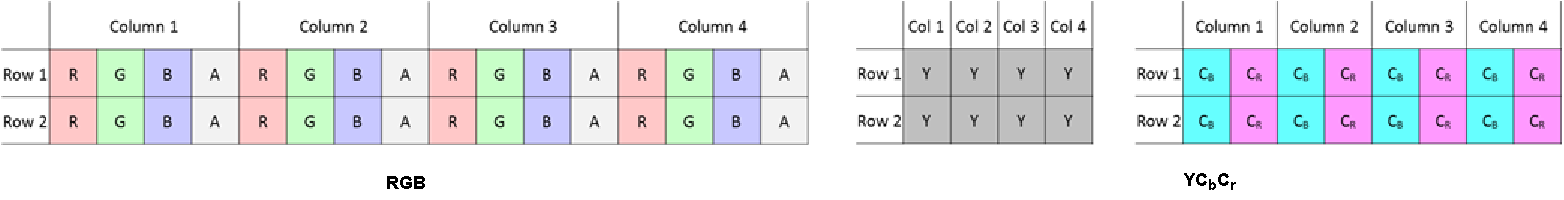
\includegraphics[width=\linewidth]{immagini/RGB_YCbCr_matrix}
	\caption{Matrice di memorizzazione di RGB e di YCbCr}
	\label{fig:RGB_YCbCr_matrix}
\end{figure}

Come detto precedentemente la codifica può essere sia software che hardware, per quanto riguarda la codifica software nel paragrafo \ref{subsec:cap3_FFmpeg} parleremo della libreria FFmpeg che supporta la codifica e decodifica di tutti i codec presenti in Tab. \ref{table:CodecsVideo} e Tab. \ref{table:CodecsAudio}, invece per la codifica hardware è importante sottolineare quali soluzioni hardware hanno utilizzato le varie piattaforme di cloud gaming.

La prima società che modificò una scheda video adattandola per il cloud gaming fu Sony che incluse un chip di codifica sulle GPU Nvidia ed AMD (rispettivamente per il rendering PS3 e PS4) \parencite{PlayStation_Now_Chip}. Altre piattaforme di cloud gaming che usano schede video con funzionalità di encoding incluse sono "Nvidia GeForce Now" su schede Nvidia \parencite{GeForce_Now}, "Microsoft XBox Cloud Gaming" su schede AMD \parencite{xCloudBlade}, "Google Stadia" su AMD \parencite{Google_Stadia_Server} e "Amazon Luna" su Nvidia \parencite{Amazon_Luna_GPU}. La lista delle aziende che creano schede video con questa funzionalità è riportata in Tab. \ref{table:VideoCardEncodingFeature} \parencite{GCNArchitecture} \parencite{IntelQuickSyncVideo} \parencite{NVIDIAVideoCodecSDK} \parencite{Hexagon_DSP_SDK}.

\begin{table}[H]
	\centering
	\begin{tabular}{||l l l||} 
		\hline
		Produttore & Funzionalità & Codec supportati \\
		\hline\hline
		AMD & Video Core Next & AVC, HEVC \\
		\hline
		Intel & Quick Sync Video & AVC, HEVC, MPEG-2, VP8, VP9 \\
		\hline
		Nvidia & NVENC & AVC, HEVC \\
		\hline
		Qualcomm & Hexagon & AVC, HEVC, H.263, MPEG-4, VP8, VP9 \\
		\hline
	\end{tabular}

	\caption{Schede video con funzionalità di codifica video}
	\label{table:VideoCardEncodingFeature}
\end{table}

Una varietà di codec audio e video sono stati implementati fino ad oggi con licenza proprietaria o libera e caratteristiche diverse. Una lista dei codec video più utilizzati\footnote{I codec video più utilizzati sono di categoria interframe.} è mostrata in Tab. \ref{table:CodecsVideo} \parencite{WebVideoCodecGuide}.

\begin{table}[H]
	\centering
	\begin{tabular}{||l l l r l||} 
		\hline
		Codec & Contenitore & Perdita dei dati & Max bit-rate\tablefootnote{In Mbps.} & Licenza\tablefootnote{Alla scadenza dei brevetti il software può essere utilizzato liberamente.} \\
		\hline\hline
		AV1 & MP4, WebM & sì & 800 & libera \\
		\hline
		AVC & MP4 & sì/no & arbitrario & proprietaria \\
		\hline
		HEVC & MP4 & sì & 800 & proprietaria \\
		\hline
		MPEG-1 & MPEG & sì & 1,5 & scaduta \\
		\hline
		MPEG-2 & MP4, MPEG & sì & 100 & scaduta \\
		\hline
		Theora & Ogg & sì & 2000 & libera \\
		\hline
		VP8 & Ogg, WebM & sì & arbitrario & libera \\
		\hline
		VP9 & Ogg, WebM & sì & arbitrario & libera \\
		\hline
	\end{tabular}

	\caption{Lista codec video}
	\label{table:CodecsVideo}
\end{table}



\subsection{Codificatori audio}
Come per i codificatori video anche i codificatori audio sono di tipo hardware o software. I codificatori hardware sono integrati nelle schede audio e sono in grado di trasformare il segnale da analogico a digitale e viceversa. Il segnale è rappresentato digitalmente come modulazione a impulsi codificati (PCM) e non è compresso.

\begin{figure}[H]
	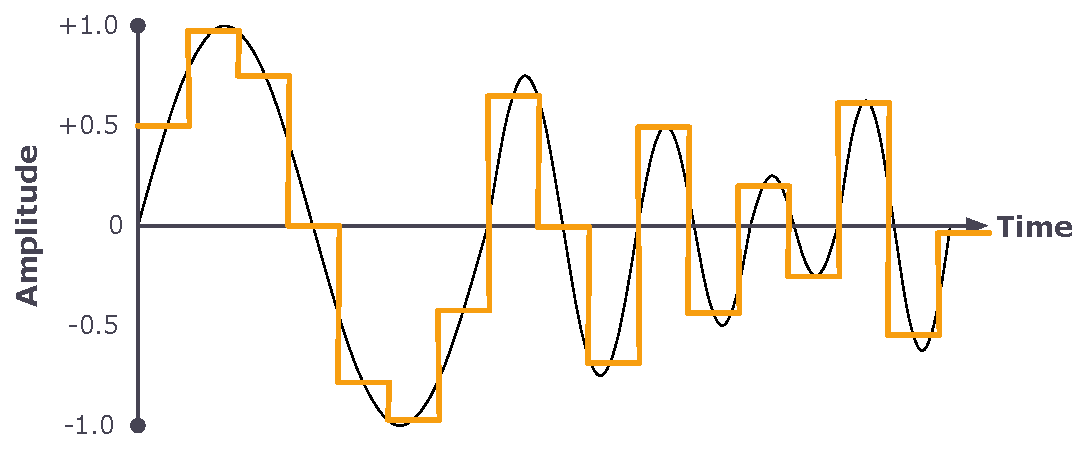
\includegraphics[width=\linewidth]{immagini/audio-waveform-samples}
	\caption{Conversione audio da analogico a digitale}
	\label{fig:audio-waveform-samples}
\end{figure}

Come mostrato in Fig. \ref{fig:audio-waveform-samples}, la linea arancione rappresenta i campioni prelevati (in questo esempio viene utilizzato il punto medio) dalla forma d'onda audio. Alla riproduzione queste ampiezze vengono utilizzate per generare un'approssimazione della forma d'onda originale. Il numero di campioni prelevati al secondo è chiamato frequenza di campionamento.

Esistono diversi formati per rappresentare i campioni all'interno di un file audio: naturali a 8 bit (uchar), interi a 16 bit (short), interi a 32 bit (int), reali a 32 bit (float) e reali a 64 bit (double); sia \textit{planar}\footnote{\textit{Planar}: ogni canale audio si trova su un piano dati separato. Tutti i piani dati hanno la stessa dimensione.} che \textit{packed}\footnote{\textit{Packed}: viene utilizzato un unico piano dati e i campioni per ciascun canale vengono interlacciati.}.

La compressione audio avviene solo tramite codificatori software. Anche questi hanno tre formati di codifica: con perdita, senza perdita e nessuna compressione. Il formato di codifica audio con perdita (l'unico usato per lo streaming) riduce la risoluzione in bit del suono e rimuove le frequenze che l'essere umano non può sentire o sente poco (secondo un modello psicoacustico). Altri fattori che influenzano la dimensione dell'audio codificato sono il numero di canali (che influisce solo sulla percezione della direzionalità e non sulla qualità) e il numero di campioni disponibili al secondo (che influiscono sulla fedeltà audio codificata) \parencite{AudioSignalProcessingAndCoding}.


%Ci sono vari algorimi base per la compressione di cui due sono maggiormente usati nei codificatori audio per lo streaming: \textit{Modified discrete cosine transform} (MDCT) e \textit{Sub-band coding} (SBC). La MDCT è una trasformata lineare ortogonale lappata, basata sull'idea della cancellazione dell'aliasing nel dominio del tempo. \parencite{AudioSignalProcessingAndCoding}.


Una lista dei codec audio più utilizzati è mostrata in Tab. \ref{table:CodecsAudio} \parencite{WebAudioCodecGuide}.

\begin{table}[H]
	\centering
	\begin{tabular}{||l l l r l||} 
		\hline
		Codec & Contenitore & Perdita dei dati & Max bit-rate\tablefootnote{In Kbps.} & Licenza\tablefootnote{Alla scadenza dei brevetti il software può essere utilizzato liberamente.} \\
		\hline\hline
		AAC & ADTS, MP4 & sì & 512 & proprietaria \\
		\hline
		ALAC & MP4 & no & variabile & proprietaria \\
		\hline
		FLAC & FLAC, MP4, Ogg & no & variabile & libera \\
		\hline
		MP2 & MPEG & sì & 320 & scaduta \\
		\hline
		MP3 & ADTS, MP4, MPEG & sì & 320 & scaduta \\
		\hline
		Opus & MP4, Ogg, WebM & sì & 510 & libera \\
		\hline
		PCM & WAV & no & 64 & scaduta \\
		\hline
		Vorbis & Ogg, WebM & sì & 500 & libera \\
		\hline
	\end{tabular}

	\caption{Lista codec audio}
	\label{table:CodecsAudio}
\end{table}


\subsection{La codifica tramite le librerie di FFmpeg} \label{subsec:cap3_FFmpeg}
Il progetto FFmpeg è un insieme di librerie e programmi open source per la gestione di video, audio, file e flussi. Include i codec per la codifica e la decodifica della maggior parte dei formati di file audio e video conosciuti \parencite{FFmpeg_Documentation}. FFmpeg include sette librerie per il C:

\begin{itemize}
	\item \verb|SW Resample| offre funzioni per il ricampionamento audio;
	\item \verb|SW Scale| offre funzioni per il ridimensionamento dell'immagine video e le routine di conversione dello spazio colore e del formato pixel;
	\item \verb|AV Codec| contiene tutti i codificatori e decodificatori audio/video FFmpeg nativi;
	\item \verb|AV Format| contiene demuxer e muxer per formati di contenitori audio e video;
	\item \verb|AV Util| è una libreria di supporto contenente routine comuni a diverse parti di FFmpeg, come funzioni hash, cifratura, decompressore LZO e codificatore/decodificatore Base64;
	\item \verb|AV Filter| permette di modificare o esaminare il video/audio tra il decoder e l'encoder;
	\item \verb|Post Proc| è una libreria contenente le vecchie routine di post-elaborazione video basate su h263.
\end{itemize}

La classe che si occupa della codifica è \verb|encode_to_movie| che utilizza le seguenti librerie FFmpeg: \verb|SW Scale| per la conversione dal modello RGB a YCbCr, \verb|SW Resample| per il ricampionamento audio, \verb|AV Codec| per la codifica audio e video e \verb|AV Format| per l'incapsulamento nel contenitore. \verb|encode_to_movie| è stata programmata per codificare in vari formati, come mostrato in Tab. \ref{table:PossibiliCodifiche}, anche se per motivi di decodifica si è scelto MPEG-TS (di cui parleremo nel paragrao \ref{sec:cap3_MPEG}).

\begin{table}[H]
	\centering
	\begin{tabular}{||l l l l l||} 
		\hline
		Contenitore & Codec video & Codec audio & Modello colore & Modello audio \\
		\hline\hline
		MP4 & AVC & AAC & YCbCr & float, planare \\
		\hline
		MPEG-TS & MPEG-1 & MP2 & YCbCr & short \\
		\hline
		WebM & VP9 & Vorbis & YCbCr & float, planare \\
		\hline
	\end{tabular}

	\caption{Lista dei codificatori utilizzabili}
	\label{table:PossibiliCodifiche}
\end{table}

Come mostrato in Fig. \ref{fig:class_server_and_encoding} il costruttore di \verb|encode_to_movie| richiede il parametro \verb|socket| su cui verrà inviato il filmato al client. Tramite le funzioni \verb|add_frame| e \verb|add_instant| vengono aggiunti il frame video e quello audio per essere codificati.

Al termine di ogni fase di incapsulamento la libreria \verb|AV Format| invia alla funzione di callback \verb|encode_to_movie::write_packet| il pacchetto (\verb|buf| di lunghezza \verb|buf_size|) appena codificato, che viene scritto sulla \verb|socket|. 

\begin{figure}[H]
	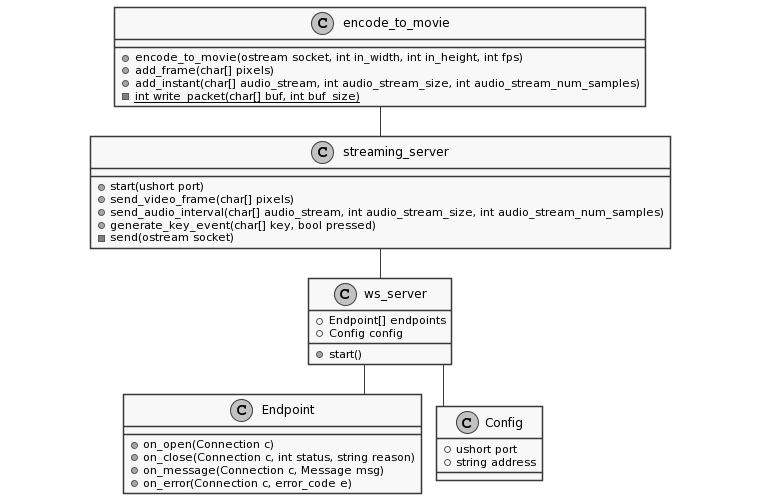
\includegraphics[width=\linewidth]{immagini/class_server_and_encoding}
	\caption{Diagramma delle classi relativo alla codifica}
	\label{fig:class_server_and_encoding}
\end{figure}



\subsubsection{Codifica video con FFmpeg}
Con riferimento al List. \ref{lst:videoCodecFFmpeg}, la codifica video inizia trasformando il frame video da SDL (\verb|uint8_t[] pixels|) al frame video FFmpeg (\verb|AVFrame|) tramite la funzione \verb|avpicture_fill|. Come detto precedentemente i codificatori video funzionano sul modello di colore YCbCr, la conversione da RGB avviene tramite la funzione \verb|sws_scale|; al termine di questa operazione \verb|yuv_frame| conterrà il frame convertito in YCbCr. Tramite le funzioni \verb|avcodec_send_frame| e \verb|avcodec_receive_packet| si comunica alla libreria FFmpeg di voler codificare il frame YCbCr. Tramite la funzione \verb|av_interleaved_write_frame| avviene la multiplazione del pacchetto video nel formato contenitore.

\begin{lstlisting}[caption=Codice per la codifica video. File: \detokenize{lib/util/encoding/encode_to_movie.hpp}, label={lst:videoCodecFFmpeg}]
void add_frame(uint8_t[] pixels)
{
	// Riempimento AVPicture con frame generato da SDL
	avpicture_fill(
		rgb_frame, 						// output
		pixels, 						// input
		AV_PIX_FMT_BGR32,				// formato input
		width, height); 				// dimensione input

	// conversione da RGB a YUV
	sws_scale(
		video_converter_context,		// contesto conversione
		rgb_frame->data,				// input
		rgb_frame->linesize, 0, height,	// dimesione input
		yuv_frame->data, 				// output
		yuv_frame->linesize); 			// dimensione output
	
	av_init_packet(&video_packet);		// pacchetto video

	// inizio codifica
	avcodec_send_frame(
		video_codec_context,			// contesto codifica
		yuv_frame);						// frame YCbCr

	// fine codifica
	avcodec_receive_packet(
		video_codec_context,			// contesto codifica
		&video_packet);					// pacchetto video

	// multiplazione pacchetto video
	av_interleaved_write_frame(
		muxer_context,					// contesto multiplazione
		&video_packet);					// pacchetto video
}
\end{lstlisting}



\subsubsection{Codifica audio con FFmpeg}
Con riferimento al List. \ref{lst:audioCodecFFmpeg}, la codifica audio inizia trasformando il frame audio da SDL (\verb|uint8_t[] stream|) al frame audio FFmpeg tramite la funzione \verb|avcodec_fill_audio_frame|. Tramite la funzione \verb|swr_convert| si converte dal formato audio SDL (PCM rappresentato tramite interi a 16 bit con segno per ogni canale) al formato audio di destinazione (come riportato in Tab. \ref{table:PossibiliCodifiche}). La funzione \verb|avcodec_fill_audio_frame| viene utilizzata nuovamente per riempire il frame audio FFmpeg con i dati appena convertiti (\verb|convertedData|). Tramite la funzione \verb|avcodec_encode_audio2| si comunica alla libreria FFmpeg di voler codificare il frame audio. Tramite la funzione \verb|av_interleaved_write_frame| avviene la multiplazione del pacchetto audio nel formato contenitore.

Tramite la funzione \verb|avformat_write_header|, che scrive l'intestazione per il flusso e alloca i dati del contesto, ha inizio la multiplazione del pacchetto audiovisivo. Questa termina chiamando la funzione \verb|av_write_trailer| che scrive il trailer per il flusso, genera il pacchetto e libera i dati del contesto; questa funzione chiama internamente la callback \verb|write_packet| di cui abbiamo parlato precedentemente, che andrà a scrivere sulla nostra \verb|socket| il pacchetto.

\begin{lstlisting}[caption=Codice per la codifica audio. File: \detokenize{lib/util/encoding/encode_to_movie.hpp}, label={lst:audioCodecFFmpeg}]
void add_instant(uint8_t[] stream, int stream_size,	int num_samples)
{
	wav_frame->nb_samples = num_samples;
	// Riempimento frame con audio da SDL
	avcodec_fill_audio_frame(
		wav_frame,						// output
		2,								// canali input
		AV_SAMPLE_FMT_S16,				// formato input
		stream,							// input
		stream_size);					// dimensione input			

	// conversione audio
	swr_convert(
		audio_converter_context,		// contesto audio
		&convertedData,					// output
		output_frame->nb_samples,		// campioni output
		wav_frame->data,				// input
		wav_frame->nb_samples);			// campioni input

	// riempimento frame destinazione
	avcodec_fill_audio_frame(
		output_frame, 					// output
		2,								// canali output
		audio_codec_context->sample_fmt,// formato output
		convertedData,					// input
		buffer_size);					// dimensione input			
			
	av_init_packet(&audio_packet);		// pacchetto audio	
	// codifica
	avcodec_encode_audio2(
		audio_codec_context,			// contesto codifica
		&audio_packet,					// pacchetto audio
		output_frame_frame);			// output			
	
	// multiplazione pacchetto audio
	av_interleaved_write_frame(
		muxer_context,					// contesto multiplazione
		&audio_packet);					// pacchetto audio
}
\end{lstlisting}



\section{Trasmissione}
La trasmissione è la fase del cloud gaming che influisce maggiormente sulla latenza e l'unica ad avere un tempo d'esecuzione condizionato dalla qualità della connessione dell'utente. Nel paragrafo \ref{subsec:cap1_StoriaDelCloudGaming} abbiamo parlato delle piattaforme che hanno fatto parte del panorama del cloud gaming, come mostrato in Tab. \ref{table:PiattaformeDiCloudGaming} i protocolli di trasmissione più usati sono stati UDP e RTP. Come detto nel paragrafo \ref{sec:cap2_SistemaProposto} in questo progetto si è scelto di utilizzare come protocollo di comunicazione WebSocket.

\subsection{WebSocket}
WebSocket è un insieme di standard formato dalle API WebSocket implementate dai browser web ed dal protocollo di comunicazione WebSocket. Il protocollo di comunicazione fornisce canali di comunicazione full-duplex su una singola connessione TCP. È supportato nativamente da tutti i browser e il suo utilizzo è simile alle normali socket. Per questi motivi è il protocollo di comunicazione generico più utilizzato sul web.

\subsubsection{WebSocket: le API}
Come mostrato nel Lis. \ref{lst:WebSocketAPI} tratto da \parencite{High_Performance_Browser_Networking} le API WebSocket fornite dal browser sono relativamente semplici. La connessione viene creata istanziando la classe \verb|WebSocket|, al costruttore oltre al URL di una risorsa WebSocket è possibile passare un vettore di stringhe che specificano dei sotto-protocolli definiti dall'utente. La classe \verb|WebSocket| espone 4 callback: errore, chiusura, apertura e ricezione messaggio. Tramite la proprietà \verb|binaryType| si può controllare il tipo di dati binari utilizzati per la ricezione (di tipo \verb|Blob| o \verb|ArrayBuffer|). La classe \verb|WebSocket| espone solo due metodi: \verb|close| per chiudere la connessione e il metodo asincrono \verb|send| per inviare dati (di tipo \verb|String|, \verb|Blob|, \verb|ArrayBuffer| o \verb|ArrayBufferView|) \parencite{WebSocket_Web_APIs}.

\begin{lstlisting}[language=JavaScript, caption=Esempio di codice delle API WebSocket, label={lst:WebSocketAPI}]
var ws = new WebSocket('ws://www.maionemiky.it/mamecgp', 
	['protocollo_utente1', 'protocollo_utente2']);

ws.binaryType = 'arraybuffer'; // or 'blob';

ws.onerror = function (error) { ... } 
ws.onclose = function () { ... } 

ws.onopen = function () { 
	ws.send('Connection established. Hello server!'); 
}

ws.onmessage = function(msg) { 
	if(msg.data instanceof ArrayBuffer)
		processArrayBuffer(msg.data);
	else if(msg.data instanceof Blob)
		processBlob(msg.data);
	else
		processText(msg.data);	
}
\end{lstlisting}

\subsubsection{WebSocket: il protocollo}
Il protocollo WebSocket è composto da due componenti: l'handshake utilizzato per negoziare i parametri della connessione, ed un meccanismo di framing dei messaggi binari per consentire un basso sovraccarico \parencite{High_Performance_Browser_Networking}.

Per stabilire la connessione il client invia una richiesta di handshake prestabilita (come mostrato in Lis. \ref{lst:Handshake_CLI}) a cui il server risponde (come mostrato in Lis. \ref{lst:Handshake_SRV}). All'interno della richiesta vengono specificati opportuni campi. Il client invia un guid casuale codificato in base64 nel campo \verb|Sec-WebSocket-Key| a cui il server riponde restituendo lo stesso guid con l'aggiunta di una costante\footnote{La stringa magica utilizzata è definita in RFC 6455.} codificando il tutto con SHA-1 prima e base64 poi. Al termine di questa procedura la comunicazione full-duplex può iniziare \parencite{Writing_WebSocket_servers}. L'implementazione server all'interno del progetto è mostrata nel Lis. \ref{lst:Handshake} relativo alla classe \verb|SocketServerBase|.

\begin{lstlisting}[language=HTML, caption=Richiesta handshake da parte del client, label={lst:Handshake_CLI}]
GET /mamecgp HTTP/1.1
Host: www.maionemiky.it
Upgrade: websocket
Connection: Upgrade
Sec-WebSocket-Key: x3JJHMbDL1EzLkh9GBhXDw==	
Sec-WebSocket-Protocol: cloudgaming
Sec-WebSocket-Version: 13
Origin: http://www.maionemiky.it
\end{lstlisting}

\begin{lstlisting}[language=HTML, caption=Risposta handshake da parte del server, label={lst:Handshake_SRV}]
HTTP/1.1 101 Switching Protocols
Upgrade: websocket
Connection: Upgrade
Sec-WebSocket-Accept: HSmrc0sMlYUkAGmm5OPpG2HaGWk=
Sec-WebSocket-Protocol: cloudgaming
\end{lstlisting}

\begin{lstlisting}[caption=Codice per handshake implementato in SocketServerBase. File: \detokenize{lib/util/server_ws_impl.hpp}, label={lst:Handshake}]
bool generate_handshake(Connection &c, ostream &handshake)
{
	auto ws_magic_string =
		"258EAFA5-E914-47DA-95CA-C5AB0DC85B11";
	auto header_it = 
		connection->header.find("Sec-WebSocket-Key");	
	auto sha1 =
		sha1_encode(header_it->second + ws_magic_string);

	handshake
		<< "HTTP/1.1 101 Web Socket Protocol Handshake" << endl
		<< "Upgrade: websocket" << endl
		<< "Connection: Upgrade" << endl
		<< "Sec-WebSocket-Accept: "
		<< base64_encode(sha1) << endl << endl;
	return true;
}
\end{lstlisting}

Come detto precedentemente WebSocket implementa un meccanismo di framing dei messaggi binari che consente la comunicazione orientata ai messaggi. Quando viene inviato un messaggio il destinatario riceve una notifica quando l'intero messaggio è stato ricevuto. Questo meccanismo divide ogni messaggio in più frame, mostrato in Fig. \ref{fig:dataframe_websocket}, che vengono trasportati, riassemblati e poi viene inviata una notifica al destinatario \parencite{High_Performance_Browser_Networking}.

Le parti più importanti che compongono un frame sono:

\begin{itemize}
	\item \textit{FIN} che indica se è l'ultimo frame;
	\item \textit{Opcode} che indica il tipo di messaggio: testo (1), binario (2), chiusura connessione (8), ping (9) e pong (10);
	\item \textit{mask} indica se il \textit{payload} è mascherato (i messaggi dal client al server hanno questo bit a 1);
	\item \textit{lunghezza payload} indica quanto è lungo il \textit{payload}: 7 bit, 7+16 bit o 7+64 bit;
	\item \textit{masking-key} contiene un valore a 32 bit usato per masherare il \textit{payload}.
\end{itemize}

\begin{figure}[H]
	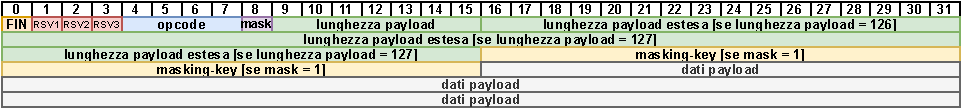
\includegraphics[width=\linewidth]{immagini/dataframe_websocket}
	\caption{Frame del WebSocket}
	\label{fig:dataframe_websocket}
\end{figure}

Con riferimento alla Fig. \ref{fig:class_server_and_encoding_full}, la classe che si occupa di inizializzare il server e comunicare con la classe per la codifica è \verb|streaming_server| la quale utilizza la classe \verb|ws_server| per comunicare tramite il protocollo WebSocket con la pagina HTML.

La classe \verb|ws_server| implementa la classe generica \verb|SocketServer| tipizzandola come socket TCP della libreria Asio\footnote{Asio è una libreria open source per la programmazione di rete.}.

\verb|SocketServer| che eredita da \verb|SocketServerBase| implementa solo il metodo \verb|accept| utilizzato per accettare una nuova connessione, come mostrato nel Lis. \ref{lst:SocketServer_accept}.

\begin{lstlisting}[caption=Funzione accept della classe SocketServer. File: \detokenize{lib/util/server_ws_impl.hpp}, label={lst:SocketServer_accept}]
void accept() override
{
	auto connection = new Connection(new SocketType(io_context));
	acceptor->accept(connection->socket);
	read_handshake(connection);
}
\end{lstlisting}

\verb|SocketServerBase| offre le funzioni per avviare e fermare il server, gestire la connessione, scrivere e leggere tramite socket e gestire l'handshake.

La classe \verb|SocketServerBase| espone gli stessi quattro eventi delle API WebSocket che vengono gestiti da \verb|SocketServerBase| ed utilizzati da \verb|streaming_server|, come mostrato in Lis. \ref{lst:SocketServer_AllCallbacks}:

\begin{itemize}
	\item \textit{open}: viene avviato il thread per eseguire l'emulazione del gioco selezionato;
	\item \textit{close}: viene spenta la macchina emulata;
	\item \textit{error}: viene stampato a video il messaggio d'errore, dopodiché il browser spegne la connessione e si verifica l'evento \textit{close};
	\item \textit{message}: alla ricezione di un messaggio viene gestito tramite la funzione \verb|process_key| l'input utente oppure il meccanismo di pausa dell'emulazione in caso di bit-rate insufficiente (è meglio mettere in pausa che far perdere il giocatore).
\end{itemize}

\begin{lstlisting}[caption=Codice relativo alle callback WebSocket. File: \detokenize{lib/util/streaming_server.hpp}, label={lst:SocketServer_AllCallbacks}]
endpoint.on_open = [this](auto connection)
{
	game_thread = new thread(on_accept, connection->parameters);
};

endpoint.on_close = [this](auto connection,
	auto status, auto reason)
{
	machine->schedule_exit();
};	

endpoint.on_error = [](auto connection, auto code)
{
	std::cout
		<< "-Error on connection from "
		<< connection->remote_endpoint_address << ":"
		<< connection->remote_endpoint_port << std::endl << ": "
		<< code.message() << std::endl;
};

endpoint.on_message = [this](auto connection, auto message)
{
	const auto msg = message->string();
	const auto values = split(msg, ":");

	if (values[0] == "ping")
		process_pausing_mechanism();
	else if (values[0] == "key")
		process_key(values);
};
\end{lstlisting}

Nel \verb|main| del programma è implementata la funzione \verb|on_accept| che avvia l'emulazione della macchina arcade selezionata, come mostrato in Lis. \ref{lst:sdlmain_callback}.

\begin{lstlisting}[caption=Codice relativo alla callback di avvenuta connessione. File: osd/sdl/sdlmain.cpp, label={lst:sdlmain_callback}]
streaming_server::instance().on_accept = [&](auto parameters)
{
	main_sdl(argc, argv, parameters["game"]);
};
\end{lstlisting}

\begin{figure}[H]
	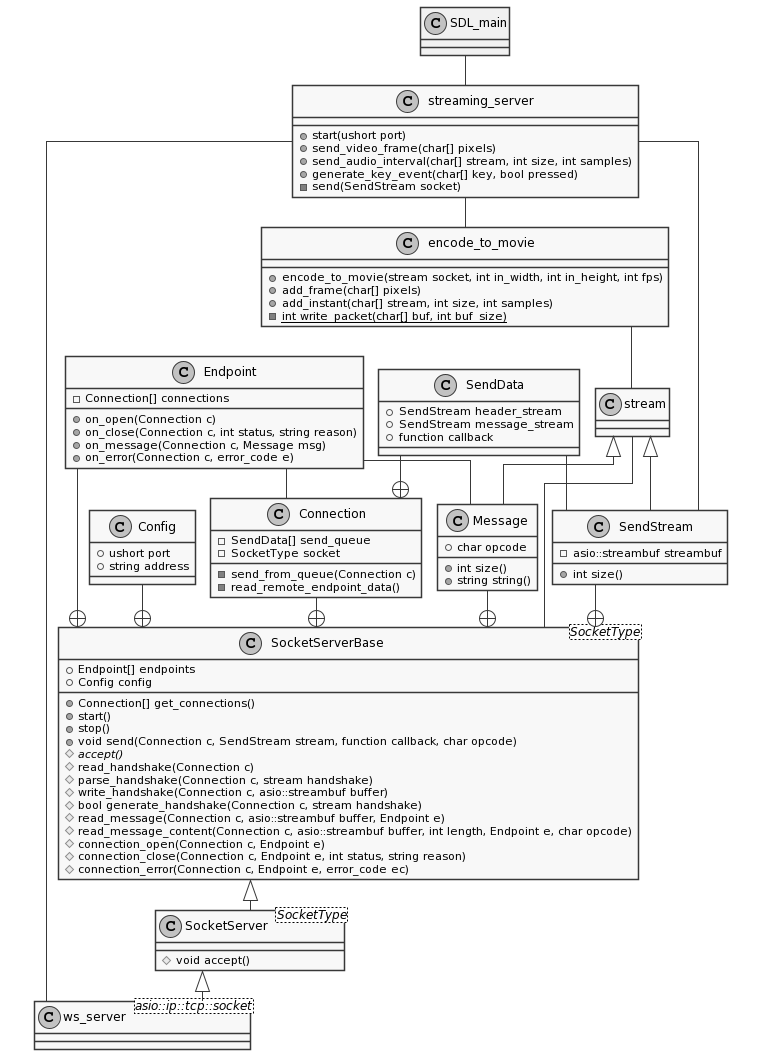
\includegraphics[width=\linewidth]{immagini/class_server_and_encoding_full}
	\caption{Diagramma delle classi del server}
	\label{fig:class_server_and_encoding_full}
\end{figure}




\section{Decodifica}
Nel paradigma del cloud gaming la decodifica viene eseguita lato client. Questa fase è vincolata dai codec installati sul sistema operativo del giocatore, per questo motivo quasi tutte le piattaforme di cloud gaming, come mostrato in Tab. \ref{table:ClientPerCloudGaming}, necessitano dell'installazione di un software client proprietario. Amazon Luna e Google Stadia, che utilizzano la tecnologia WebRTC, sono attualmente le uniche piattaforme ad offrire la possibilità di poter giocare tramite il browser (solo Chrome è supportato). Come detto precedentemente questo progetto mira ad offrire il più semplice accesso alla piattaforma, per questo motivo si è scelto come client il browser web e quindi la fase di decodifica viene eseguita dal browser utilizzando una libreria JavaScript.

\begin{table}[H]
	\centering
	\begin{tabular}{||l l l l||} 
		\hline
		Piattaforma & Protocollo & Installazione app. & Client \\
		\hline\hline
		Amazon Luna & RTP & sì/no & Chrome, iOS, Android \\
		\hline
		GeForce Now & RTP & sì & Windows, macOS, Android \\
		\hline
		Google Stadia & RTP & sì/no & Chrome, iOS, Android \\
		\hline
		MAME CGP & WebSocket & no & Browser \\
		\hline
		Playkey & UDP & sì & Windows, macOS \\
		\hline
		PlayStation Now & UDP & sì & PS4, PS5, Windows \\
		\hline
		Vortex & UDP & sì & Windows, macOS, Android \\
		\hline		
		Xbox Cloud Gaming & UDP & sì & Android \\
		\hline
	\end{tabular}

	\caption{Piattaforme disponibili}
	\label{table:ClientPerCloudGaming}
\end{table}

I moderni browser web offrono due API per la grafica, le Canvas API e WebGL, e le Web Audio API per la riproduzione sonora.

Le Canvas API forniscono un mezzo per disegnare grafica tramite JavaScript, si concentrano principalmente sulla grafica 2D ma quando vengono utilizzate dalle API WebGL possono disegnare grafica 2D e 3D con accelerazione hardware. Sono completamente supportate da tutti i browser \parencite{Canvas_API}.

WebGL è una API JavaScript, progettata e gestita dal gruppo no-profit Khronos, per il rendering di grafica 2D e 3D. WebGL 1.0 è supportato da tutti i browser, mentre WebGL 2.0 è in fase di testing \parencite{WebGL}.

Su queste API sono state create delle librerie JavaScript per la decodifica di vari formati audiovisivi.

\subsection{Le librerie JavaScript per la decodifica} \label{subsec:chap3_LibJavascript}
Per questo progetto sono state provate varie librerie open-source:

\begin{itemize}
	\item \textit{jMuxer} per la decodifica audiovisiva dei formati AVC e AAC. Necessita di due stream separati, uno per l'audio ed uno per il video;	
	\item \textit{ogv.js} in grado di decodificare i seguenti formati audiovisivi open-source: Vorbis, Theora, Opus, VP8, VP9 e AV1;
	\item \textit{JSMpeg} in grado di decodificare il formato MPEG-TS con i codec MPEG-1 per il video e MP2 per l'audio.
\end{itemize}

\textit{jMuxer}, come mostrato nel Lis. \ref{lst:example_jMuxer}, richiede che lo stream audio e video siano separati e che venga specificata la durata in millisecondi del pacchetto audio/video.
 
\begin{lstlisting}[language=JavaScript, caption=Esempio di utilizzo di jMuxer, label={lst:example_jMuxer}]
let player = new JMuxer({
	node: 'myCanvas',
	mode: 'both', // available values are: both, audio and video
});

player.feed({
	audio: audio,
	video: video,
	duration: duration // in ms
});
\end{lstlisting}

La libreria \textit{ogv.js}, come mostrato nel Lis. \ref{lst:example_ogv}, è anche essa molto semplice da usare ed è in grado di decodificare molti formati open-source; purtroppo nella versione attuale può leggere solamente file completi.
 
\begin{lstlisting}[language=JavaScript, caption=Esempio di utilizzo di ogv.js, label={lst:example_ogv}]
let player = new OGVPlayer();

myCanvas.appendChild(player);

player.src = URL;
player.play();
\end{lstlisting}

\textit{JSMpeg} si è rivelato relativamente facile da usare. Come mostrato nel Lis. \ref{lst:example_JSMpeg}, si possono specificare le dimensioni del buffer video e di quello audio. Questa funzionalità è stata molto utile per ridurre l'effetto di latenza percepito dall'utente, poiché non è possibile usare buffer nel paradigma del cloud gaming. La libreria è in grado di acquisire il filmato tramite connessione WebSocket (questa operazione ha richiesto una modifica al sorgente della libreria).

\begin{lstlisting}[language=JavaScript, caption=Esempio di utilizzo di JSMpeg, label={lst:example_JSMpeg}]
let player = new JSMpeg.Player(URL, {
	canvas: 'myCanvas',
	autoplay: true,
	loop: false,
	pauseWhenHidden: false,
	videoBufferSize: 64 * 1024,
	audioBufferSize: 48 * 1024,
});
\end{lstlisting}

La scelta finale è ricaduta su \textit{JSMpeg} sia perché offre le funzionalità per gestire i buffer sia perché supporta il protocollo WebSocket. \textit{JSMpeg} è una libreria composta da un demuxer MPEG-TS, un decoder video MPEG-1 e audio MP2, con un sistema di rendering basato sia su WebGL che su Canvas2D, ed un sistema di output audio basato su Web Audio. Consente lo streaming a bassa latenza ($\sim$50ms) tramite WebSocket, ed è rilasciata con licenza MIT \parencite{JSMpeg}. MPEG verrà descritto nel paragrafo \ref{sec:cap3_MPEG}.




\section{Cattura dell'input utente}
L'ultima fase del cloud gaming è la cattura dell'input utente da inviare al server. Questa fase viene eseguita lato client, nel nostro caso sarà il browser ad eseguirla. MAME CGP consente di poter giocare sia tramite tastiera che tramite joystick a più giocatori sullo stesso dispositivo. Per far ciò sono state utilizzate due librerie JavaScript open source per la gestione dell'input:

\begin{itemize}
	\item Keypress è una libreria per la cattura dell'input da tastiera specializzata per l'uso in contesti videoludici, rilasciata con licenza Apache 2.0 \parencite{Keypress};
	\item GameController.js è una libreria che estende le Web API per il gamepad, rilasciata con licenza MIT \parencite{gameController_js}.
\end{itemize}

Come mostrato nel Lis. \ref{lst:InitInput}, tratto dal file \verb|MAME.js|, la funzione \verb|InitKeyboard| si occupa di inizializzare la libreria Keypress e la funzione \verb|InitGamepad| la libreria GameController. I tasti mappati sono: le quattro direzioni, gli otto tasti azione e i tasti funzione start, gettone e pausa. Nel listato è mostrata la mappatura del tasto pausa per la tastiera e del tasto R2 per il joystick. In ambedue i casi deve essere gestita la pressione e il rilascio.

\begin{lstlisting}[language=JavaScript, caption=Codice relativo alla gestione input lato client. File: \detokenize{Streaming/HTML/MAME.js}, label={lst:InitInput}]
function InitKeyboard()
{
	keypress_Listener = new window.keypress.Listener();

	if (!keypress_Listener)
		return; // tastiera non presente

	keypress_Listener.register_many([
		{
			"keys": "p",
			"on_keydown": ()=> InputSend(keyboard, 'PAUSE', true),
			"on_keyup": (e)=> InputSend(keyboard, 'PAUSE', false),
		},
		// continua ...
	]);
}

function InitGamepad()
{
	gameControl.on('connect', gamepad =>
	{
		gamepad.before('r2', ()=> InputSend(gamepad.id, 'R2', true));
		gamepad.after('r2', ()=> InputSend(gamepad.id, 'R2', false));
		// continua ...
	}
}
\end{lstlisting}


\subsection{Invio dell'input alla libreria SDL}
Come detto nel paragrafo \ref{subsec:cap2_GestioneInput} l'input è gestito tramite la libreria SDL. Come mostrato nel Lis. \ref{lst:SocketServer_AllCallbacks} alla ricezione di un messaggio di tipo "key" il server chiama la funzione \verb|process_key| che si occupa di analizzare i dati contenuti nel messaggio e chiamare la funzione \verb|generate_key_event|, mostrata nel Lis. \ref{lst:generate_key_event}, che invia alla classe device l'input ricevuto tramite WebSocket. Nel Lis. \ref{lst:sdl_keyboard_device} è mostrata l'unica modifica apportata alla classe \verb|sdl_keyboard_device| che serve a passare per riferimento il device SDL alla classe \verb|streaming_server|.

\begin{lstlisting}[caption=Codice relativo alla gestione input lato server: modulo server. File: \detokenize{lib/util/streaming_server.hpp}, label={lst:generate_key_event}]
void generate_key_event(char[] key, bool down)
{
	SDL_Event e;
	e.type = down ? SDL_KEYDOWN : SDL_KEYUP;
	e.key.keysym.scancode = SDL_GetScancodeFromName(key);
	e.key.keysym.sym = SDL_GetKeyFromScancode(e.key.keysym.scancode);

	keyboard->queue_events(&e, 1);
}
\end{lstlisting}

\begin{lstlisting}[caption=Codice relativo alla gestione input lato server: modulo SDL. File: \detokenize{osd/modules/input/input_sdl.cpp}, label={lst:sdl_keyboard_device}]
// costruttore
sdl_keyboard_device(running_machine &r, char[] n, char[] id,
	input_module &m): sdl_device(r, n, id, DEVICE_CLASS_KEYBOARD, m)
{
	streaming_server::instance().set_keyboard(this);
}
\end{lstlisting}




\section{MPEG-1} \label{sec:cap3_MPEG}
MPEG-1 è uno standard (ISO/IEC 11172) del \textit{Moving Pictures Experts Group} del 1991 per la compressione audiovisiva con perdita. È stato progettato per lo standard NTSC (240p a 30 fps) per un bit-rate di 1,5 Mbit/s ma supporta risoluzioni fino a $4095\times4095$ px ed un bit-rate fino a 100 Mbit/s. In questo progetto è stato utilizzato con una risoluzione di 480p a 30fps per un bit-rate massimo di 2,1 Mbit/s (dipende dalla dinamicità delle schermate del gioco e dalla presenza di musica); questa impostazione può essere cambiata a riga di comando come mostrato nel paragrafo \ref{sec:chapMU_Esecuzione}. Di seguito vedremo il processo di codifica video ed audio e il trasporto.



\subsection{Video}
Un filmato \textit{MPEG-1 Video} è suddiviso in 6 layer, come mostrato in Fig. \ref{fig:MPEG_layers}, su cui si applicano dei processi di codifica e decodifica formati da vari algoritmi. Il processo di codifica, mostrato in Fig. \ref{fig:mpegPhases}, utilizza l'algoritmo di compressione (con perdita) JPEG:

\begin{enumerate}
    \item L'immagine viene elaborata in blocchi da $8\times8$ px;
    \item Viene applicata, su ogni blocco, la trasformata discreta del coseno (DCT) prima orizzontalmente e poi verticalmente;
    \item Ogni blocco viene compresso tramite quantizzazione.
\end{enumerate}

\begin{figure}[H]
	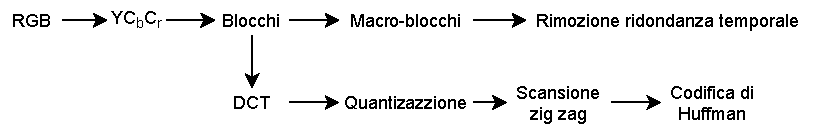
\includegraphics[width=\linewidth]{immagini/mpegPhases}
	\caption{Fasi della codifica video}
	\label{fig:mpegPhases}
\end{figure}

Il processo completo di codifica e decodifica è mostrato in Fig. \ref{fig:MPEGCodingScheme}.

\begin{figure}[H]
	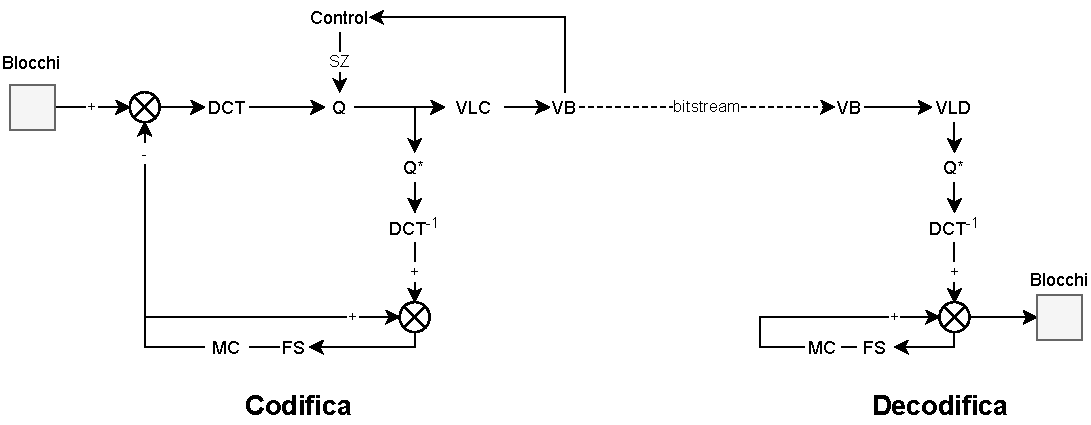
\includegraphics[width=\linewidth]{immagini/MPEGCodingScheme}
	\centering
	\caption{\textit{MPEG-1 Video}: schema di codifica e decodifica}
	\label{fig:MPEGCodingScheme}
\end{figure}



\subsubsection{Frame e macroblocchi}
In \textit{MPEG-1 Video} la sequenza video è composta da "gruppi di immagini" (GOP: \textit{group of pictures}); ogni GOP è composto da un \textit{I-frame}, da una sequenza di \textit{P-frame} e \textit{B-frame} e da un \textit{D-frame}, come mostrato in \ref{fig:gop}.

\begin{figure}[H]
	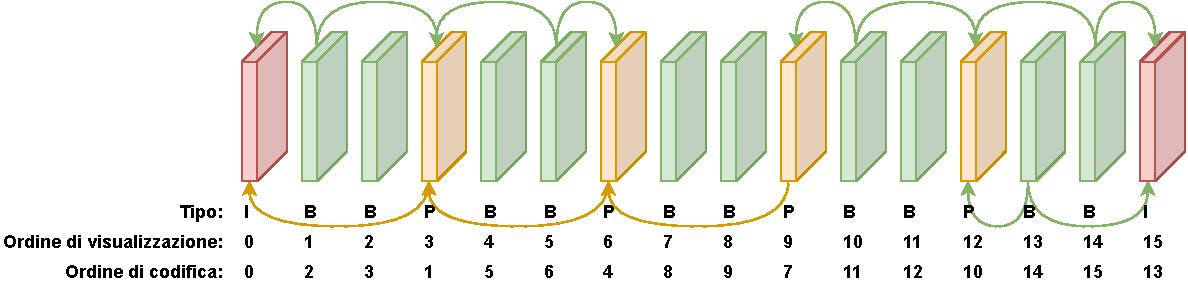
\includegraphics[width=\linewidth]{immagini/gop}
	\caption{GOP: ogni \textit{I-frame} inizia un nuovo GOP; le frecce indicano da che frame prendono informazioni}
	\label{fig:gop}
\end{figure}

Una configurzione tipica è formata da 9 frame di cui 2 \textit{P-frame} e 6 \textit{B-frame}. Ogni GOP è formato da quattro diversi tipi di frame \parencite{VideoAndMultimediaTransmissionsOverCellularNetworks}:

\begin{itemize}
	\item \textit{I-frame} (\textit{Intra-frame}) sono chiamati anche \textit{key-frame} perché sono codificati senza utilizzare informazioni diverse da quelle contenute nell'immagine stessa;
	\item \textit{P-frame} (\textit{Predicted-frame}) sfruttano la ridondanza temporale per aumentare la compressione. Memorizzano solamente le differenze nell'immagine rispetto al frame precedente;
	\item \textit{B-frame} (\textit{Bidirectional-frame}) come i \textit{P-frame} fanno una predizione però sfruttando sia il frame precedente che quello successivo;
	\item \textit{D-frame} mentre gli altri tre sono presenti in quasi tutti i codec video i \textit{D-frame} sono presenti solamente in \textit{MPEG-1 Video}. La loro funzione è di fornire un'anteprima del video in un punto (usata nei visualizzatori video). Sono frame a bassa qualità (proprio perché le anteprime solitamente sono molto piccole) ed oggi la loro funzione è stata sostituita dagli \textit{I-frame}.
\end{itemize}

\begin{figure}[H]
	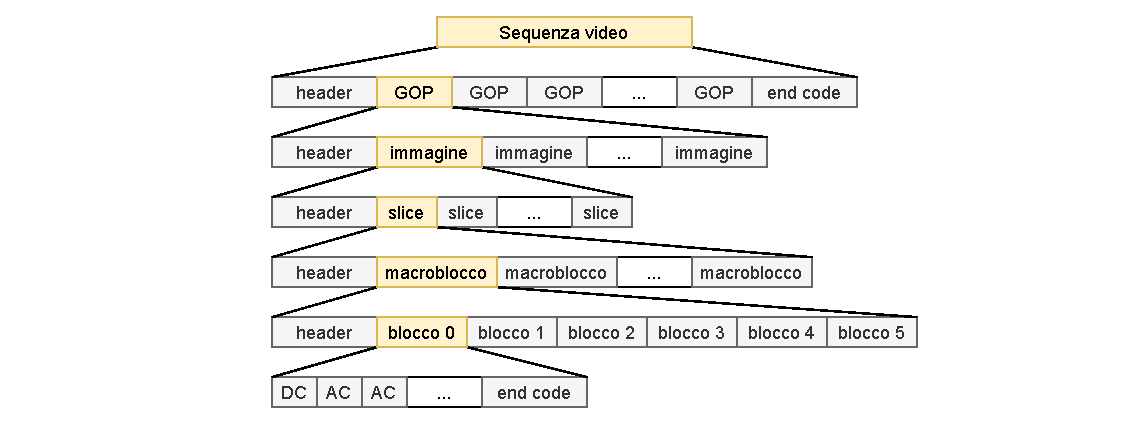
\includegraphics[width=\linewidth]{immagini/MPEG_layers}
	\caption{Layer di \textit{MPEG-1 Video}}
	\label{fig:MPEG_layers}
\end{figure}

Come mostrato in Fig. \ref{fig:MPEG_layers}, ogni immagine (frame) è divisa in \textit{slice}. Le slice sono di 3 tipi: Y, Cb e Cr. Ogni \textit{slice} è scomposta in macroblocchi, che sono l'unità d'elaborazione della compressione. I macroblocchi sono formati da $16\times16$ px e sono necessari ai fini del calcolo dei vettori di movimento e dei blocchi di errore per la compensazione del movimento. I macroblocchi a loro volta, utilizzando un campionamento 4:2:0\footnote{Il campionamento 4:2:0 riduce di un fattore 2 in ambedue le direzioni.}, sono formati da 4 blocchi per la luminanza (Y di YCbCr) e 2 per la crominanza (Cb e Cr) come mostrato in Fig. \ref{fig:macroblocchi}. Essi si dividono in \parencite{ProgettazioneEproduzioneMultimediale}:

\begin{itemize}
	\item \textit{macroblocchi I} codificato indipendentemente da altri macroblocchi (dalla trasformazione coseno discreta 2D come nei blocchi JPEG);
	\item \textit{macroblocchi P} codificare non la regione ma il vettore di movimento e il blocco di errore del fotogramma precedente (macroblocco previsto in avanti);
	\item \textit{macroblocchi B} come sopra tranne che il vettore di movimento e il blocco di errore sono codificati dal frame precedente (macroblocco previsto in avanti) o successivo (macroblocco previsto all'indietro).
\end{itemize}

\begin{figure}[H]
	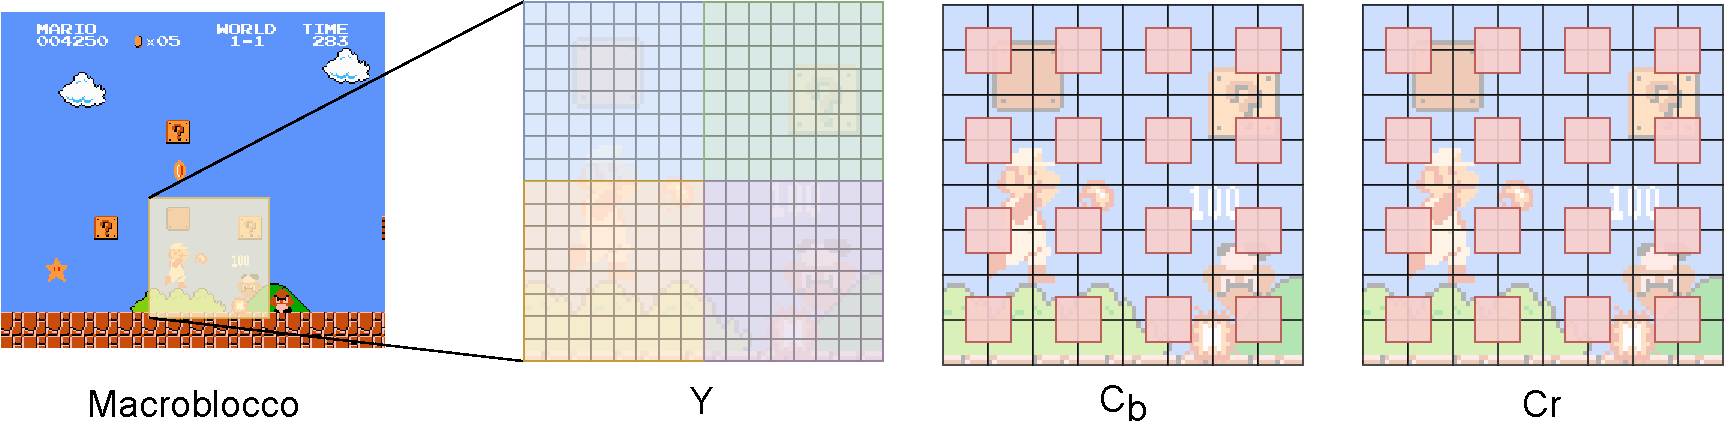
\includegraphics[width=\linewidth]{immagini/macroblocchi}
	\centering
	\caption{Disposizione blocchi per il campionamento 4:2:0}
	\label{fig:macroblocchi}
\end{figure}

I frame possono contenere differenti tipi di macroblocchi:

\begin{itemize}
	\item \textit{I-frame} contiene solamente macroblocchi \textit{I};
	\item \textit{P-frame} può contenere macroblocchi \textit{I} o \textit{P};
	\item \textit{B-frame} può contenere tutti i tipi di macroblocchi (\textit{I}, \textit{P} o \textit{B}).
\end{itemize}

Per ogni \textit{I-frame} i macroblocchi vengono ri-calcolati. Per i \textit{P-frame} e \textit{B-frame} i macroblocchi possono essere: ri-calcolati, copiati, spostati o modificati \parencite{MPEG_1_Video}.



\subsubsection{Dal dominio spaziale a quello delle frequenze: la DCT}
La trasformata discreta del coseno (DCT)\footnote{La forma più comune è la DCT-II che è quella utilizzata in questo contesto.} divide la forma d'onda nelle sue componenti frequenziali, di per se non effettua nessuna compressione ma trasforma i pixel in una forma nella quale è possibile identificare la ridondanza, poiché i coefficienti della DCT sono correlati alle frequenze spaziali dell'immagine. Inoltre non tutte le frequenze spaziali sono presenti per questo si avranno, come risultato, molti coefficienti prossimi allo zero.

I blocchi degli \textit{I-frame} sono trasformati dal dominio spaziale a quello delle frequenze utilizzando la DCT, definita in Eq. \ref{eq:DCT}, che viene eseguita sui blocchi da $8\times8$ px della luminanza e della crominanza. Questo processo divide l'immagine in parti (in sottobande spettrali) di diversa importanza \parencite{HyesookLim2000Asaf}.

\begin{equation} \label{eq:DCT}
	\begin{aligned}
		& y(k) = \sqrt{\frac{2}{N}} \cdot u(k) \cdot \sum_{n=0}^{N-1} x(n) \cdot cos \frac{(2n+1)k\pi}{2N}, & \forall k = 0, 1, \dots, N-1\\
		& u(k) =
		\begin{cases}
			\frac{1}{\sqrt{2}},	& \text{se } k=0\\
			1,					& \text{altrimenti}
		\end{cases}
	\end{aligned}
\end{equation}

%È computazionalmente più facile da implementare e più efficiente considerare la DCT come un insieme di funzioni di base che può essere precalcolato e memorizzato. In pratica si calcolano i valori per un kernel di convoluzione ($8\times8$) che verrà successivamente applicato. I valori sono calcolati dalla formula DCT.



\subsubsection{La quantizzazione e la scansione zig-zag}
Successivamente la matrice di 64 frequenze del blocco DCT viene uniformemente quantizzata (dividendo per lo \textit{step-size}) utilizzando la matrice di quantizzazione in Eq. \ref{matr:MPEG_Quant_Matrix}. Il sistema visivo umano è più sensibile agli errori di ricostruzione relativi alle frequenze spaziali più basse per questo si migliora la qualità visiva dell'immagine decodificata utilizzando dei pesi tarati sulle proprietà fisiche del sistema visivo umano. La quantizzazione è un processo che introduce perdita di qualità del segnale \parencite{ProgettazioneEproduzioneMultimediale}.

\begin{minipage}{0.5\linewidth}
	\begin{equation} \label{matr:MPEG_Quant_Matrix}
		\begin{bmatrix} 
			8 & 16 & 19 & 22 & 26 & 27 & 29 & 34\\
			16 & 16 & 22 & 24 & 27 & 29 & 34 & 37\\
			19 & 22 & 26 & 27 & 29 & 34 & 34 & 38\\
			22 & 22 & 26 & 27 & 29 & 34 & 37 & 40\\
			22 & 26 & 27 & 29 & 32 & 35 & 40 & 48\\
			26 & 27 & 29 & 32 & 35 & 40 & 48 & 58\\
			26 & 27 & 29 & 34 & 38 & 46 & 56 & 69\\
			27 & 29 & 35 & 38 & 46 & 56 & 69 & 83\\
		\end{bmatrix}
	\end{equation}
	\vfill
\end{minipage}%
\begin{minipage}{0.5\linewidth}
	\centering
	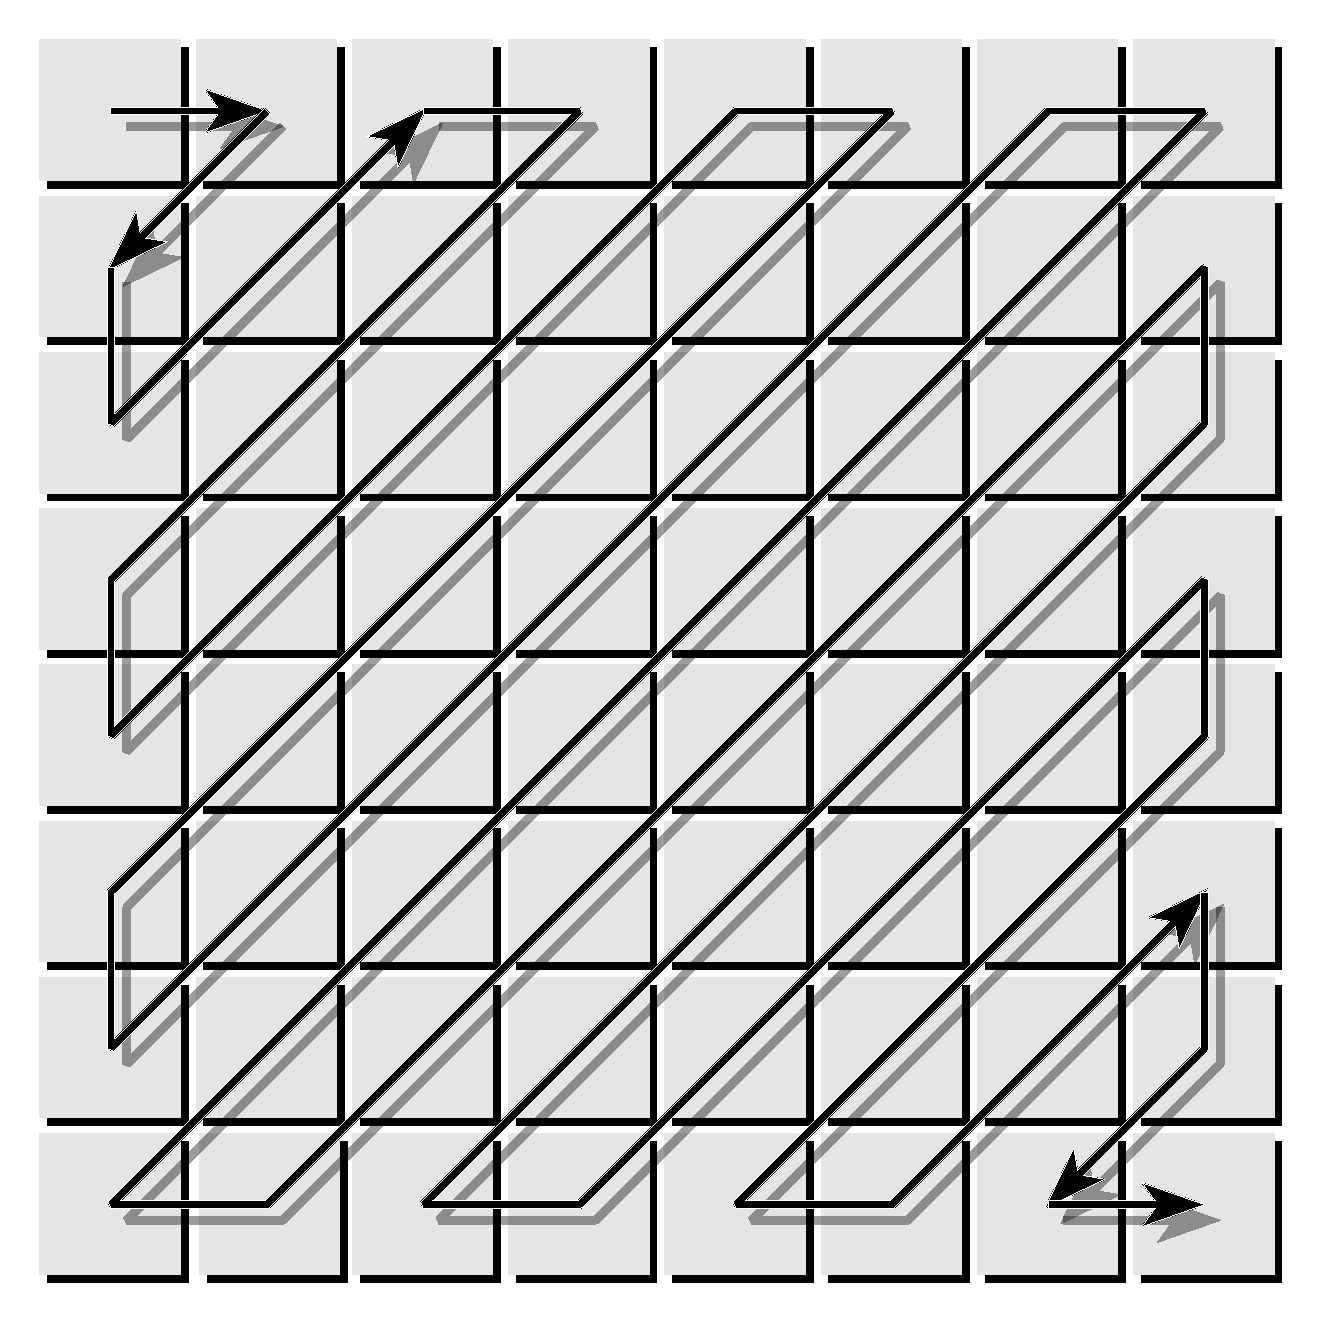
\includegraphics[width=4cm]{immagini/JPEG_ZigZag}
	\captionof{figure}{Scansione zig-zag}
	\label{fig:JPEG_ZigZag}
\end{minipage}%

Dopo la quantizzazione, il coefficiente DCT con la varianza più alta (coefficiente DC) viene trattato in modo diverso dai coefficienti rimanenti (coefficienti AC). Il coefficiente DC corrisponde all'intensità media del blocco. I valori del quantizzatore diversi da zero dei restanti coefficienti DCT vengono scansionati "a zig-zag", come mostrato in Fig. \ref{fig:JPEG_ZigZag}, e codificati con l'entropia della lunghezza di esecuzione utilizzando tabelle di "codici a lunghezza variabile". La scansione zig-zag ispeziona in successione ed in ordine crescente gli elementi.



\subsubsection{Stima predittiva e compensazione del movimento}
La stima predittiva del movimento mira a ridurre i dati trasmessi calcolando il movimento degli oggetti in una sequenza video, risparmiando tra il 50\% e il 80\% di bit da memorizzare. I passaggi di questo processo sono:

\begin{enumerate}
	\item trova il macroblocco più adatto nel frame di riferimento cercando in una determinata area, questo è il macroblocco predetto;
	\item invia i coefficienti DCT quantizzati della differenza tra i due frame, chiamata errore di predizione;
	\item codifica e invia il vettore movimento tra la posizione del macroblocco predetto e quello del frame di riferimento.
\end{enumerate}

\begin{figure}[H]
	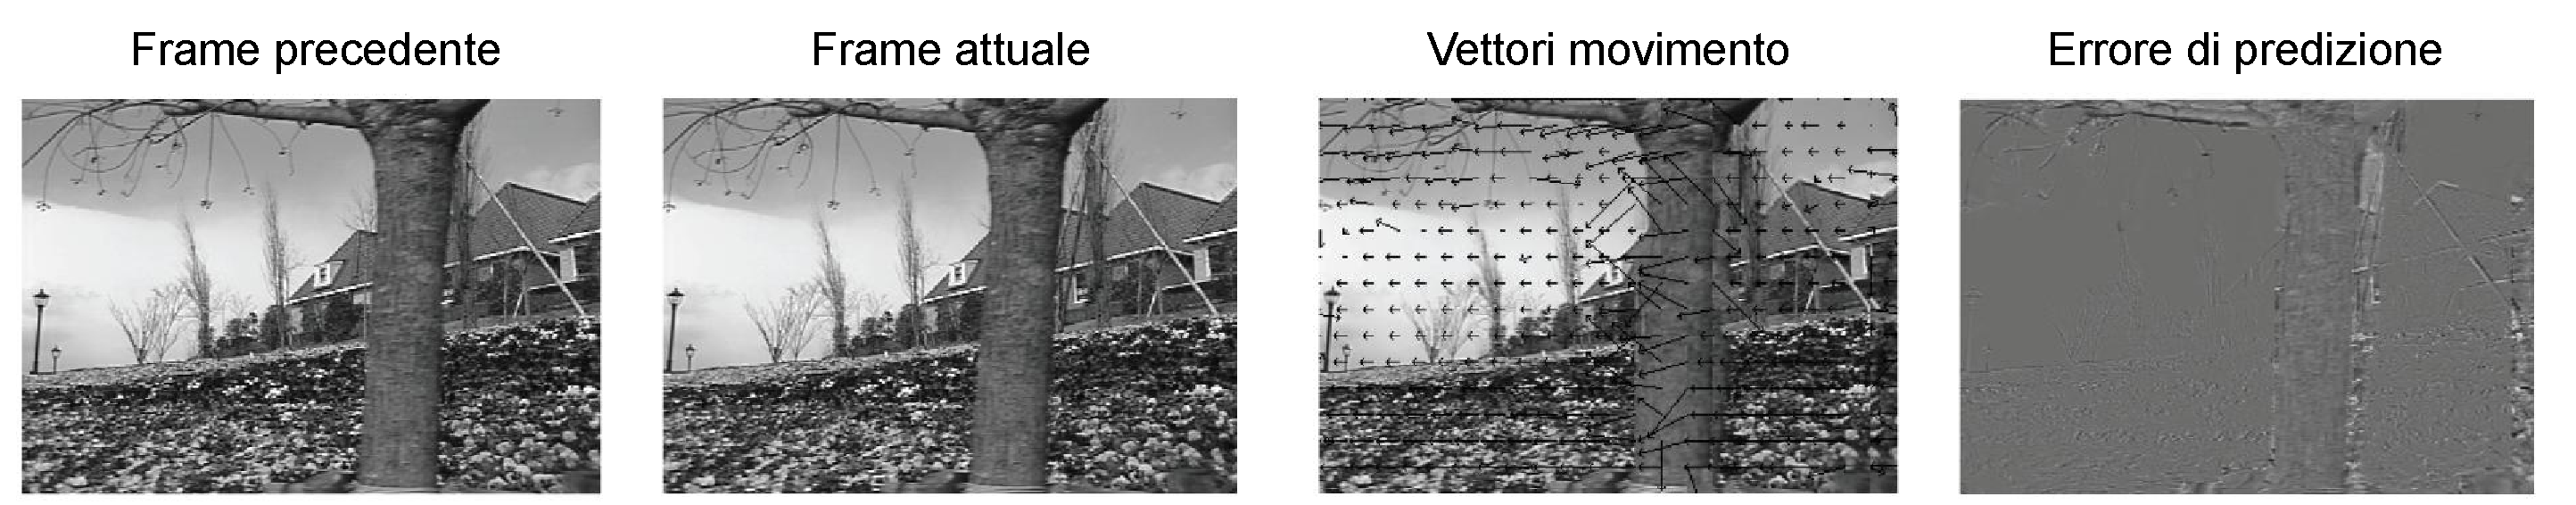
\includegraphics[width=\linewidth]{immagini/motioncompensation}
	\caption{Compensazione del movimento: vettori di movimento ed errore di predizione. Fonte: \fullcite{Computer_Vision_A_Modern_Approach}}
	\label{fig:motioncompensation}
\end{figure}

Il processo di applicare i vettori movimenti ad un frame per sintetizzare la trasformazione al frame successivo è chiamato compensazione del movimento e si applica solamente ai \textit{P-frame} e \textit{B-frame}. 

\begin{figure}[H]
	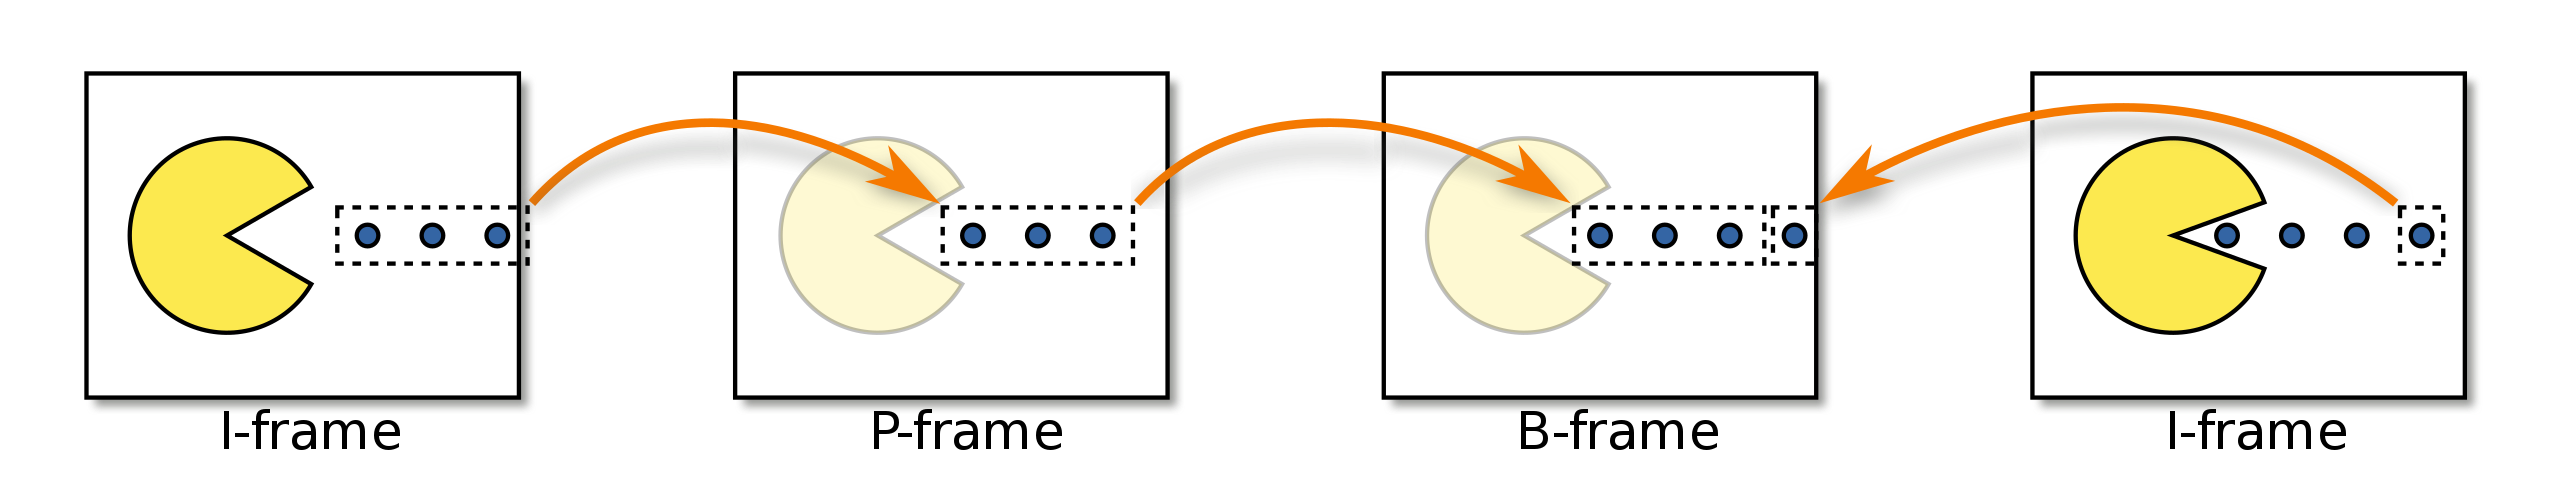
\includegraphics[width=\linewidth]{immagini/I_P_and_B_frames}
	\caption{Vettori movimento. Le frecce arancioni che partono dal frame di riferimento al frame di predizione indicano i frame che l'algoritmo prende in considerazione; le frecce rosse indicano il vettore movimento calcolato. Fonte: wikipedia.org}
	\label{fig:I_P_and_B_frames}
\end{figure}

Un esempio molto semplice dei vettori movimento è mostrato in Fig. \ref{fig:I_P_and_B_frames}, mentre in Fig. \ref{fig:motioncompensation} è mostrata la compensazione del movimento.

L'errore di predizione può essere calcolato tramite \textit{mean absolute error}, \textit{sum of squared error} o \textit{mean squared error}. Solitamente implementato utilizzando \textit{mean absolute error}, utilizzando l'Eq. \ref{eq:MAE}, dove $C_{ij}$ è il frame corrente e $R_{ij}$ quello di riferimento \parencite{ProgettazioneEproduzioneMultimediale}:

\begin{equation} \label{eq:MAE}
	\frac{1}{N^2} \sum_{i=0}^{N-1} \sum_{j=0}^{N-1} |C_{ij}-R_{ij}|
\end{equation}



\subsubsection{Run-length encoding e la codifica di Huffman}
Il \textit{run-length encoding} (RLE) è un algoritmo di compressione senza perdita di informazione. Sostituisce nell'input le sequenze di caratteri uguali con il numero di occorrenze consecutive, il carattere ed un simbolo.

Ad esempio la stringa \verb|AAAAAAFDDCCCCCCCAEEEEEEEEEEEEEEEE| diventa \verb|6A:1F:2D:7C:1A:16E|.

La codifica di Huffman è anche esso un algoritmo per la compressione senza perdita di informazione. L'algoritmo crea un albero binario di simboli ordinati in base al conteggio delle loro occorrenze. Agli elementi che si ripetono più spesso viene assegnato il codice più breve.

I coefficienti AC sono codificati senza perdite secondo il RLE e memorizzati utilizzando la codifica di Huffman, mentre i coefficienti DC codificano le differenze tra blocchi dei macroblocchi.

Al termine di queste due operazioni si ottiene il bitstream del video \parencite{jurgem_1997}.




\subsection{Audio}
\textit{MPEG-1 Audio} riduce il quantitativo di dati da utilizzare per l'audio tramite psicoacustica, eliminado frequenze che l'orecchio umano non può sentire. Lo standard sonoro è diviso in 3 layer:

\begin{itemize}
	\item Layer I: è progettato per la codifica in tempo reale tramite hardware con un bit-rate di 384 kbit/s. L'estensione del file è \verb|.m1a|;
	\item Layer II: è un formato con perdita proggettato per l'alta qualità a 192 kbit/s. L'estensione del file è \verb|.mp2|;
	\item Layer III: anche esso un formato con perdita progettato per una buona qualità a 128 kbit/s; L'estensione del file è \verb|.mp3|.
\end{itemize}

Come detto nel paragrafo \ref{subsec:chap3_LibJavascript}, la libreria \textit{JSMpeg} supporta \textit{MPEG-1 Audio Layer II (MP2)}.

\subsubsection{La tecnica di codifica}
La codifica, come mostrato in Fig. \ref{fig:mpegaudio}, opera su dati di tipo PCM a 16 bit campionati a $32$, $44,1$ o $48$ kHz, che vengono decomposti in 32 sottobande utilizzando un filterbank PQMF\footnote{PQMF: \textit{pseudo quadrature mirror filter} è un filterbank in cui la cancellazione dell'aliasing avviene solo tra bande adiacenti.}. Le sottobande sono sottoposte a compansione a blocchi dimodoché l'ampiezza massima dei campioni sia unitaria.

Parallelamente l'input PCM viene inviato ad una FFT\footnote{FFT: \textit{fast Fourier transform} (trasformata di Fourier veloce) è un algoritmo per calcolare la trasformata discreta di Fourier.} da 1024 punti, che scompone il segnale nelle sue frequenze costituenti, come mostrato in Fig. \ref{fig:FFT}. Successivamente l'analisi del segnale psicoacustico scarta tutti i suoni sotto la \textit{soglia assoluta della percezione sonora} (ATH\footnote{ATH: \textit{Absolute Threshold of Hearing}, stimata attorno i $10^{-12} W/m^{2}$.}) insieme a quelli difficilmente audibili. Quindi una procedura di allocazione dinamica dei bit (iterativa) applica la soglia di "distorsione appena rilevabile" (JND\footnote{JND: \textit{just noticeable distortion}.}) per selezionare il quantizzatore migliore da un insieme predeterminato per ciascuna sottobanda \parencite{AudioSignalProcessingAndCoding}.

\begin{figure}[H]
	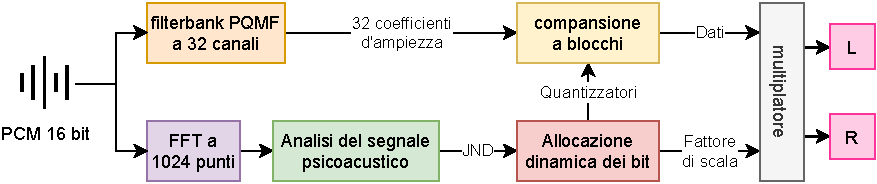
\includegraphics[width=\linewidth]{immagini/mpegaudio}
	\caption{\textit{MPEG-1 Audio}: schema di codifica}
	\label{fig:mpegaudio}
\end{figure}

\begin{figure}[H]
	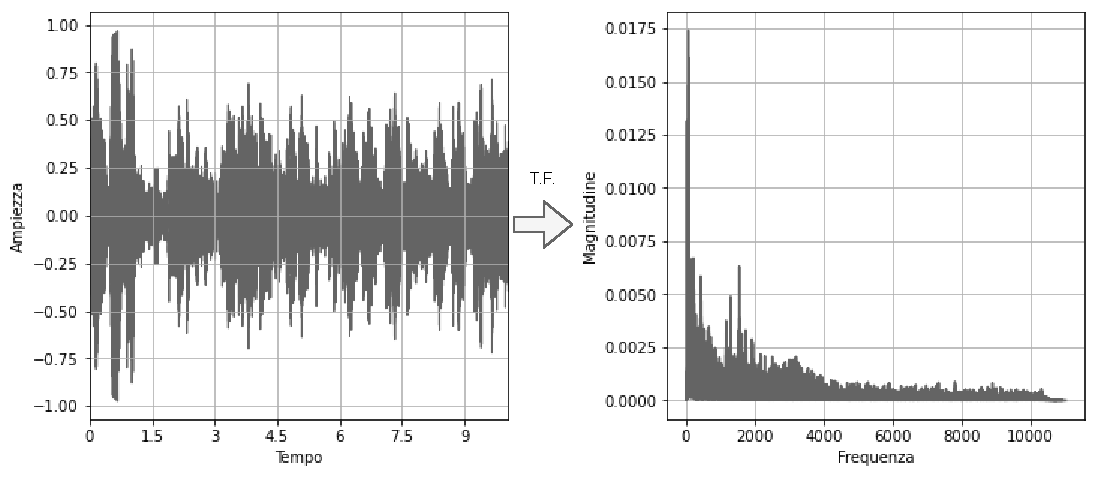
\includegraphics[width=\linewidth]{immagini/FFT}
	\caption{Applicazione della trasformata discreta di Fourier (1D) su 10 secondi di audio (PCM a 16 bit) tratti da \textit{Street Fighter III}}
	\label{fig:FFT}
\end{figure}



\subsection{Trasporto}
Il trasporto definisce il modo in cui il filmato viene compresso in byte per la trasmissione da una parte all'altra, utilizzando un protocollo. MPEG, nel layer di sistema, definisce \textit{Program Stream} (PS) e \textit{Transport Stream} (TS), il primo usato per la memorizzazione sui DVD ed il secondo per i sistemi di trasmissione per la TV via cavo. 

\textit{MPEG-TS} è composto da più flussi audio e video (PES\footnote{PES: \textit{Packetized elementary stream} definisce il trasporto dei flussi elementari (ES), cioè l'output di un codificatore audio o video.}), non necessariamente sincronizzati, che vengono multiplessati assieme e trasmessi sotto forma di pacchetti, come mostrato in Fig. \ref{fig:MPEGTS}.

\begin{figure}[H]
	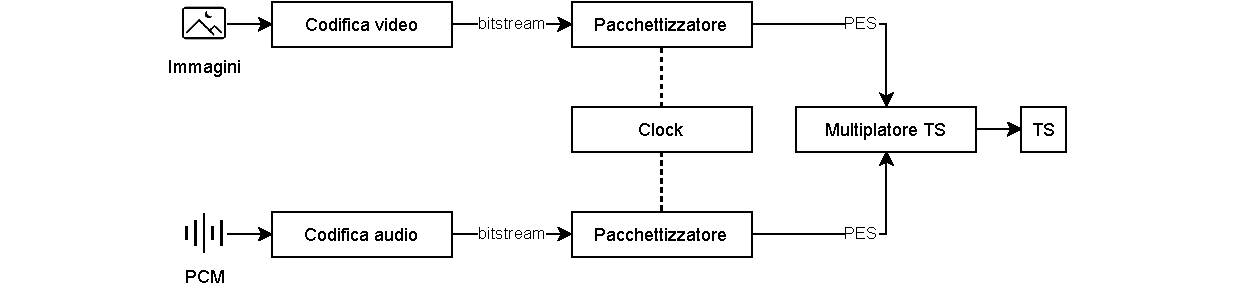
\includegraphics[width=\linewidth]{immagini/MPEGTS}
	\caption{Schema di funzionamento del \textit{Transport Stream}}
	\label{fig:MPEGTS}
\end{figure}

I pacchetti TS sono formati da un header di 4 bytes e un payload di 184 bytes, come mostrato in Fig. \ref{fig:TS_Packet}, e sono composti da \parencite{RetiInternetMultimediali}:

\begin{itemize}
    \item \textit{Synchronization Byte}: identifica l'inizio del pacchetto (è la costante 0x47);
    \item \textit{Transport Error Indicator}: indica un errore nel pacchetto;
    \item \textit{Payload Unit Start Indicator}: indica se il contenuto è un pacchetto PS;
    \item \textit{Transport priority}: indica se ha priorità sugli altri pacchetti;
    \item \textit{Packet Identifier}: identificatore del pacchetto;
    \item \textit{Transport Scrambling Control}: indica se il pacchetto è mischiato e se con chiave pari o dispari;
	\item \textit{Adaptation field control}: indica se il campo AF è settato;
    \item \textit{Continuity counter}: numero di sequenza del pacchetto;
    \item \textit{Adaptation field}: informazioni aggiuntive sul pacchetto;
\end{itemize}

\begin{figure}[H]
	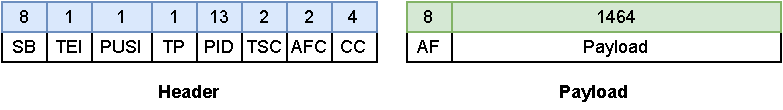
\includegraphics[width=\linewidth]{immagini/TS_Packet}
	\caption{Pacchetto \textit{MPEG-TS}}
	\label{fig:TS_Packet}
\end{figure}